
\section{Maišymo modeliavimas}

\subsection{Reakcijos stabdymo sąlyga}

Kompiuterinio modelio rezultatai rodo, kad vykstant reakcijai, reagentų kiekis erdvėje artėja prie 0, tačiau niekad jo nepasiekia. Tai būdinga ir realybėje vykstančioms reakcijoms, dėl šios priežasties kompiuterinio modelio darbą stabdysime, kai sureaguos $\eta_\text{stop}\%$ pradinių medžiagų kiekio. Matematiškai reakcijos stabdymo laiką $t_\text{stop}$ galime apibrėžti taip:

\begin{align}
    q(t_\text{stop})=\left(1-\frac{\eta_\text{stop}}{100}\right)q(0),\quad \eta_\text{stop}\in[0, 100)
\end{align}

Tolimesniems pavyzdžiams ir analizei naudosime konkrečią reikšmę $\eta_\text{stop}=97$ ir reakciją stabdysime laiku $t_\text{stop}$, kai $q(t_\text{stop})=0.03q(0)$. Toks procentas pasirinktas todėl, kad sureagavus 97\% reagentų, reakcija iš esmės yra pasibaigusi ir gautų duomenų užtenka atlikti analizei.

\subsection{Atsitiktinis maišymas}

Konstruojant kompiuterinį modelį šiam procesui atkreipsime dėmesį į kelias svarbias detales:

\begin{itemize}
  \item Išmaišymas vyksta prie daug žemesnės temperatūros negu reakcija
  \item Išmaišymas gali vykti kelis kartus
  \item Išmaišymo procesas nėra deterministinis
\end{itemize}

\paragraph{Maišymas prie žemesnės temperatūros}

Kadangi maišymas vyksta prie daug žemesnės temperatūros negu pati reakcija, darysime prielaidą, kad ištraukus reagentus iš krosnies cheminė reakcija ir difuzija nevyksta, todėl medžiagų maišymą modeliuosime kaip momentinį procesą, kuris įvyksta tarp diskrečių laiko žingsnių.

\paragraph{Maišymas kelis kartus}

Praktikoje vykdant šią reakcija chemikai savo nuožiūra pasirenka laiką, kuriuo vykdys išmaišymą, todėl ir kompiuterinis modelis turėtų suteikti vartotojui pasirinkimą nurodyti konkrečius laiko momentus, kada vyks medžiagų išmaišymas. Šiuos laikus žymėsime taip:

\begin{align}
    t^1_\text{mix}, t^2_\text{mix}, \dots, t^{T^*}_\text{mix} \quad T^*\in \mathbb{N}
\end{align}

Čia $T^*$ -- bendras išmaišymų skaičius, o $t^i_\text{mix}$ -- $i$-tojo išmaišymo laikas. Kadangi kompiuterinis modelis laiko informaciją apie diskrečius laiko taškus $t_n$, mes negalime tiesiogiai apibrėžti sąlygos, kad išmaišymas vyks konkrečiu laiko momentu $t^i_\text{mix}$, todėl medžiagas išmaišysime einamajame laiko žingsnyje $t_n$, kuris yra artimiausias išmaišymo laikui $t^i_\text{mix}$:

\begin{figure}[!h]
\centering
\label{mix-inequality-graphic}
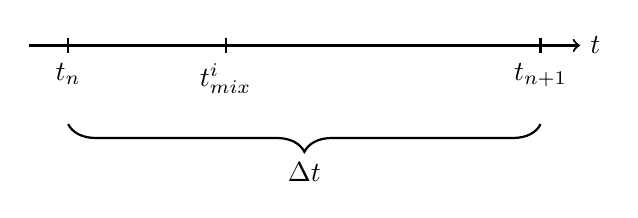
\begin{tikzpicture}[thick]

% Main timeline
\draw[->] (-0.5,0) -- (6.5,0) node[right] {$t$}; % Timeline with axis label

% Time points
\foreach \x/\label in {0/{$t_n$}, 2/{$t^i_\text{mix}$}, 6/{$t_{n+1}$}} {
    \draw (\x,0.1) -- (\x,-0.1) node[below] {\label};
}

% Braces for interval
\draw[decorate,decoration={brace,amplitude=10pt,mirror}] (0,-1) -- (6,-1) node[midway,below=10pt] {$\Delta t$};


\end{tikzpicture}
\caption{Šiuo atveju, išmaišymas įvyks laiko žingsniu $t_n$, o ne $t_{n+1}$, nes $t^i_\text{mix}$ yra arčiau laiko momento $t_n$}
\end{figure}

arba kitaip sakant išmaišymas įvyks laiko žingsniu $t_n$, jei:

\begin{align}
    \vert t_n - t^i_\text{mix} \vert < \frac{1}{2}\Delta t \label{mix-inequality}
\end{align}

\paragraph{Nedeterministinis maišymas}

Maišymas praktikoje yra chaotiškas procesas, todėl sudarydami kompiuterinį modelį turime į tai atsižvelgti. Maišymą modeliuosime kaip reakcijos erdvės sričių atsitiktinį išdėstymą. Pradinė erdvę $\Omega$ padalinsime į mažesnes, nepersidengiančias, vienodas kvadratines sritis $\Omega_i$, tada sugeneruosime atsitiktinę $4$-permutaciją $\sigma$ ir $4$ atsitiktinius kampus $\theta_i \in \{0, \frac{\pi}{2}, \pi, \frac{3\pi}{2}\}$. Kiekviena iš sričių $\Omega_i$ keliauja į poziciją, kurioje yra sritis $\Omega_{\sigma(i)}$, tačiau pasukta kampu $\theta_i$. 

\begin{figure}[!h]
\centering
\label{split-reaction-space}

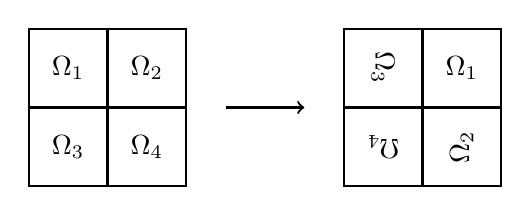
\begin{tikzpicture}
    % Original Grid
    \draw[thick] (0,0) rectangle (2,2);
    \draw[thick] (1,0) -- (1,2);
    \draw[thick] (0,1) -- (2,1);

    \node at (0.5,1.5) {$\Omega_1$};
    \node at (1.5,1.5) {$\Omega_2$};
    \node at (0.5,0.5) {$\Omega_3$};
    \node at (1.5,0.5) {$\Omega_4$};

    % Arrow
    \draw[->, thick] (2.5,1) -- (3.5,1);

    % Transformed Grid
    \begin{scope}[shift={(4,0)}]
        \draw[thick] (0,0) rectangle (2,2);
        \draw[thick] (1,0) -- (1,2);
        \draw[thick] (0,1) -- (2,1);

        \node at (0.5,1.5) {\rotatebox{270}{$\Omega_3$}}; % Rotated 180° horizontally
        \node at (1.5,1.5) {$\Omega_1$};             % No change
        \node at (0.5,0.5) {\rotatebox{180}{$\Omega_4$}}; % Upside down
        \node at (1.5,0.5) {\rotatebox{90}{$\Omega_2$}};  % 90° rotation
    \end{scope}
\end{tikzpicture}
\caption{Maišymo transformacijos pavyzdys}
\end{figure}

\newpage
\subsection{Atsitiktinio maišymo rezultatai}

\begin{figure}[h!]
\centering
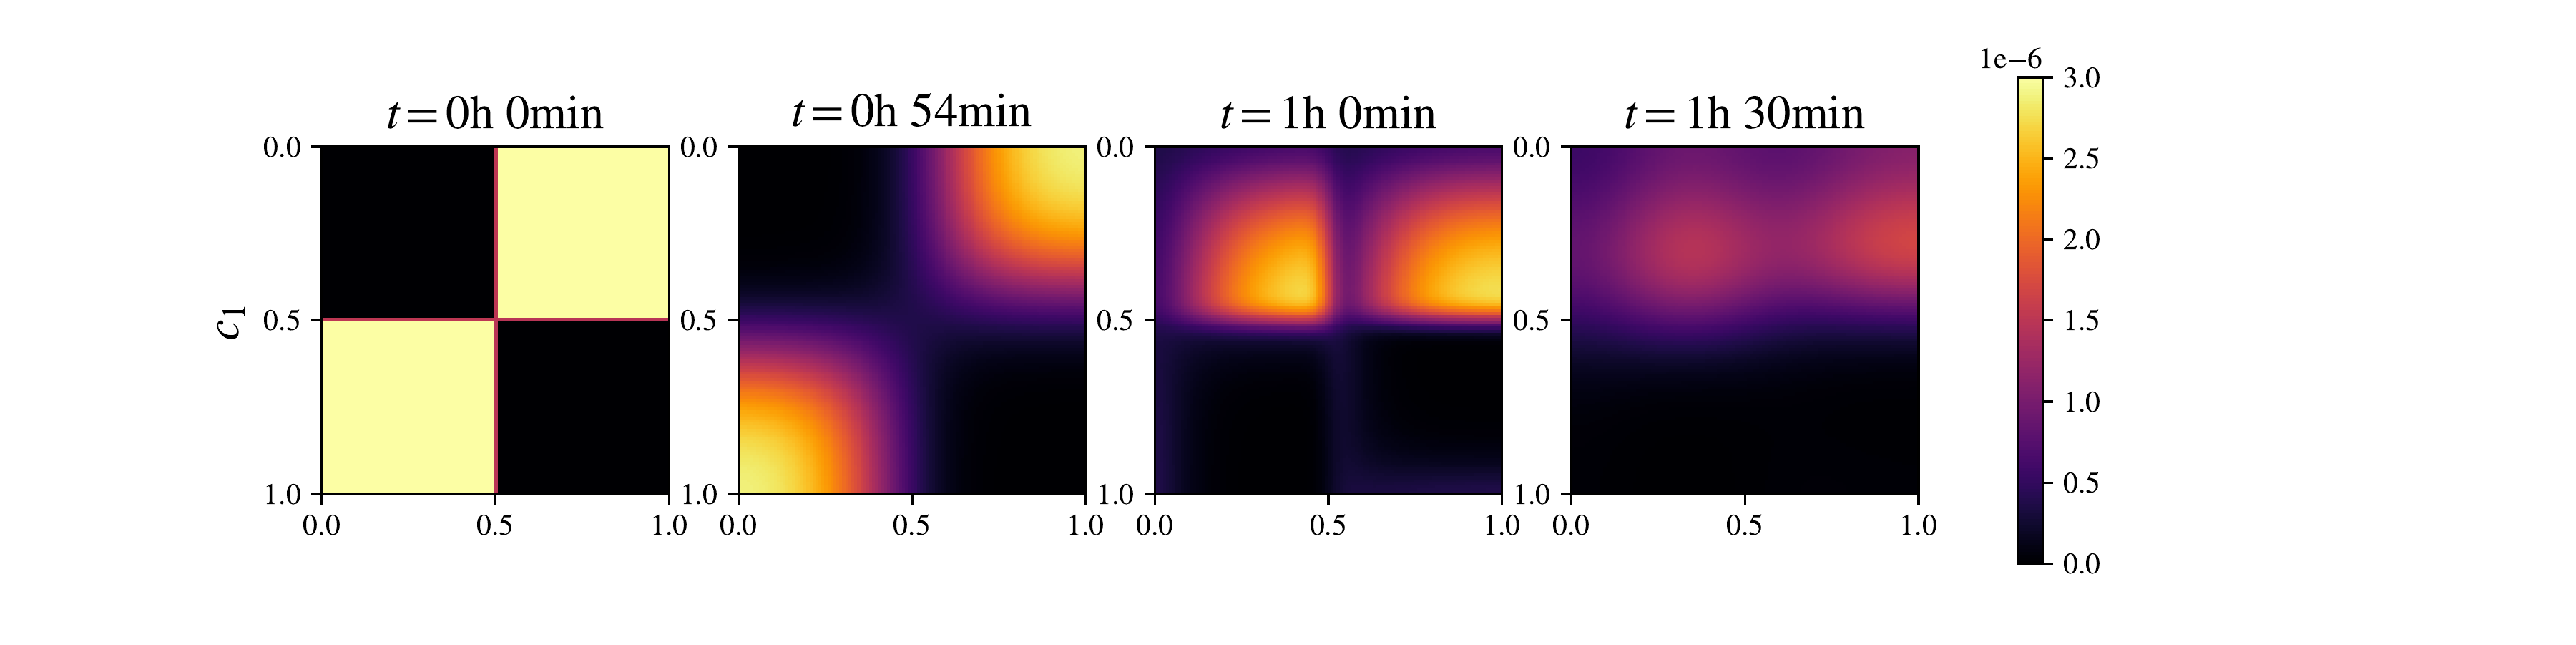
\includegraphics[width=\textwidth]{../paper/assets/random-mix-example-c0-1.png} \\
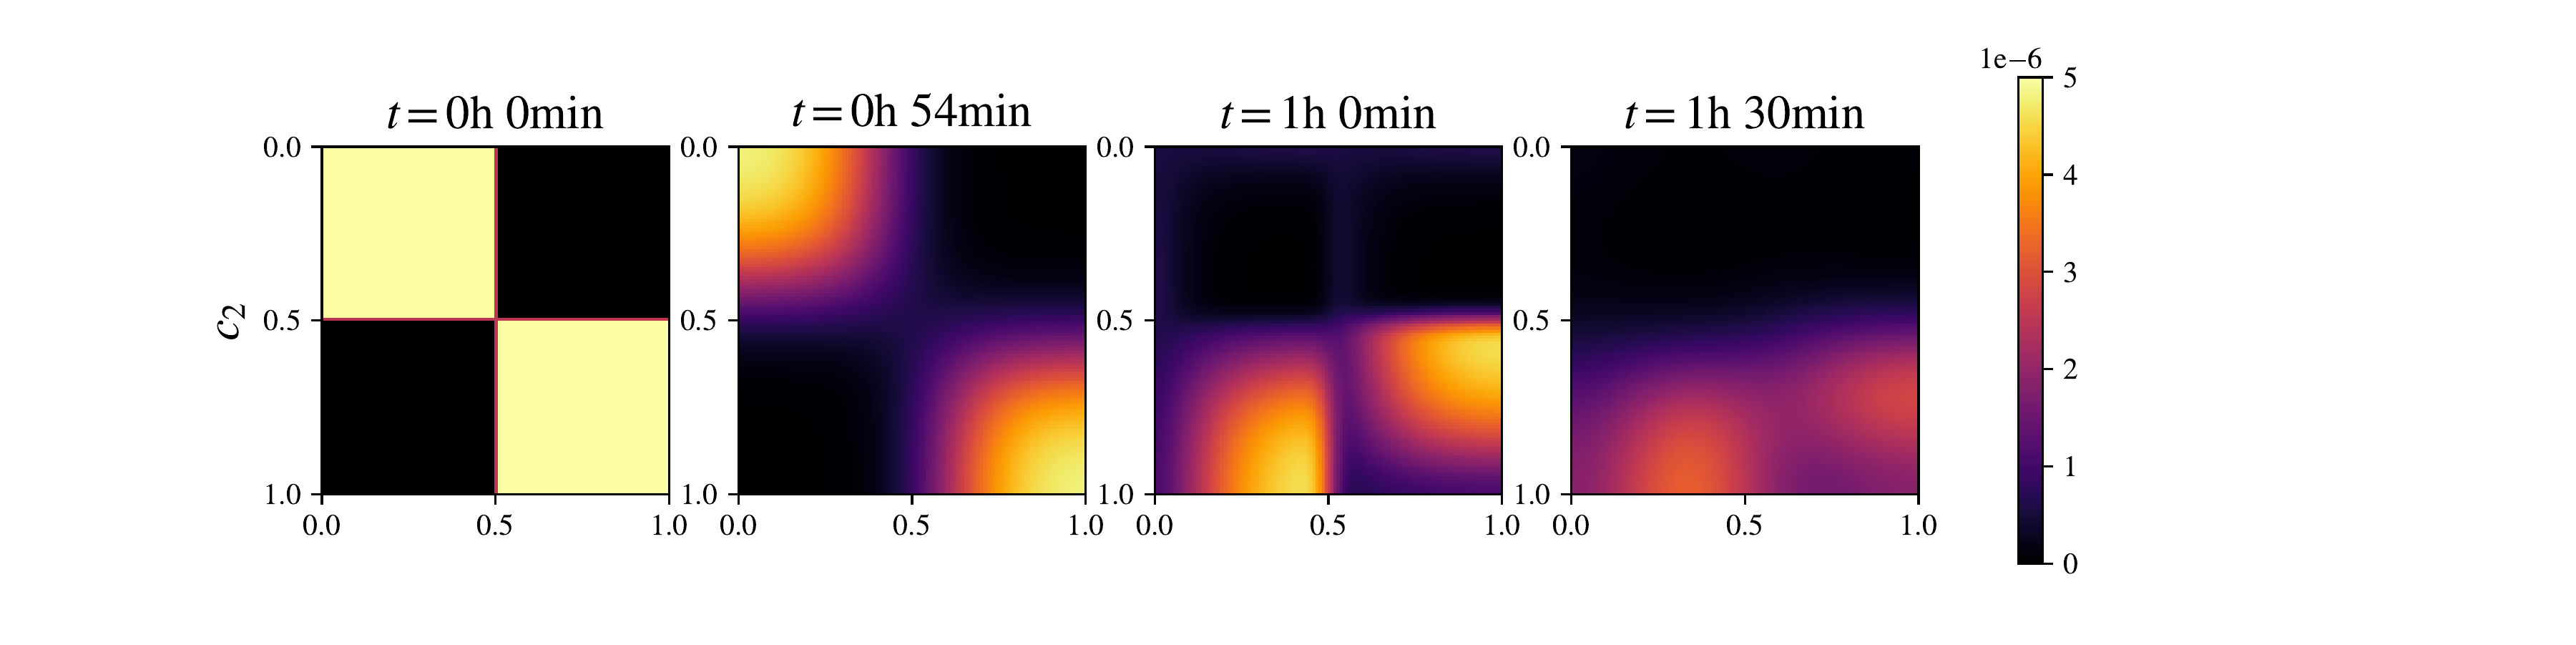
\includegraphics[width=\textwidth]{../paper/assets/random-mix-example-c1-1.png} \\
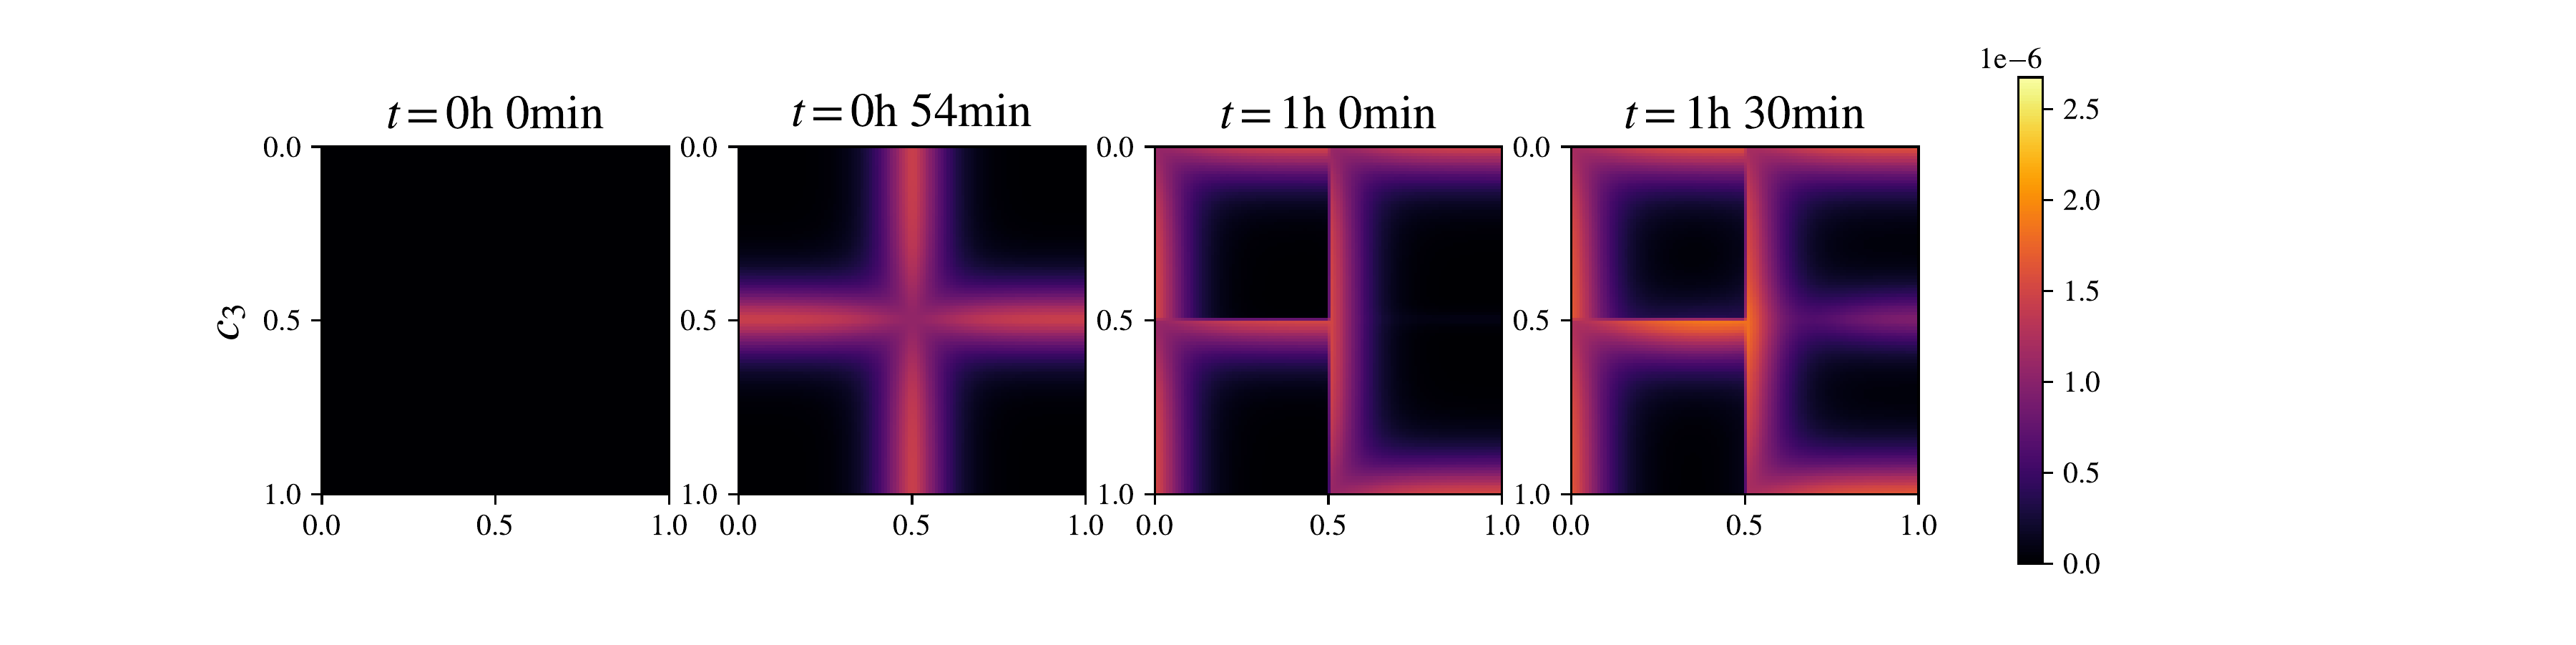
\includegraphics[width=\textwidth]{../paper/assets/random-mix-example-c2-1.png}

\caption{Kompiuterinio modelio rezultatai - medžiagų koncentracijos per laiką, kai vyksta išmaišymas. Išmaišymo laikas $t^1_\text{mix} = 1h$ }

\label{mix-example}
\end{figure}

\ref{mix-example}-ame pavyzdyje matome kaip atrodo reakcijos eiga, kada vyksta išmaišymas. Trečiame stulpelyje ir ypatingai trečios medžiagos koncentracijoje matome ryškių artefaktų. Taip yra todėl, kad nuo išmaišymo praejo labai mažai laiko ir medžiagos nespėjo sureaguoti. Čia galime pastebėti tam tikrą problemą su atsitiktiniu išmaišymu - šiuo atveju, po išmaišymo, susidarė tik viena viena sienelė, ties kuria susiduria dar nesureagavusios skirtingų medžiagų mikrodalelės, ir dėl to tarp laiko momentų $t=1h$ ir $t=1h\,30min$ matome labai nežymų pokytį trečios medžiagos $c_3$ koncentracijoje. Daugiau informacijos apie tokio išmaišymo efektus būtų galima matyti medžiagos kiekio grafike.

\newpage
\begin{figure}[h!]
    \centering
    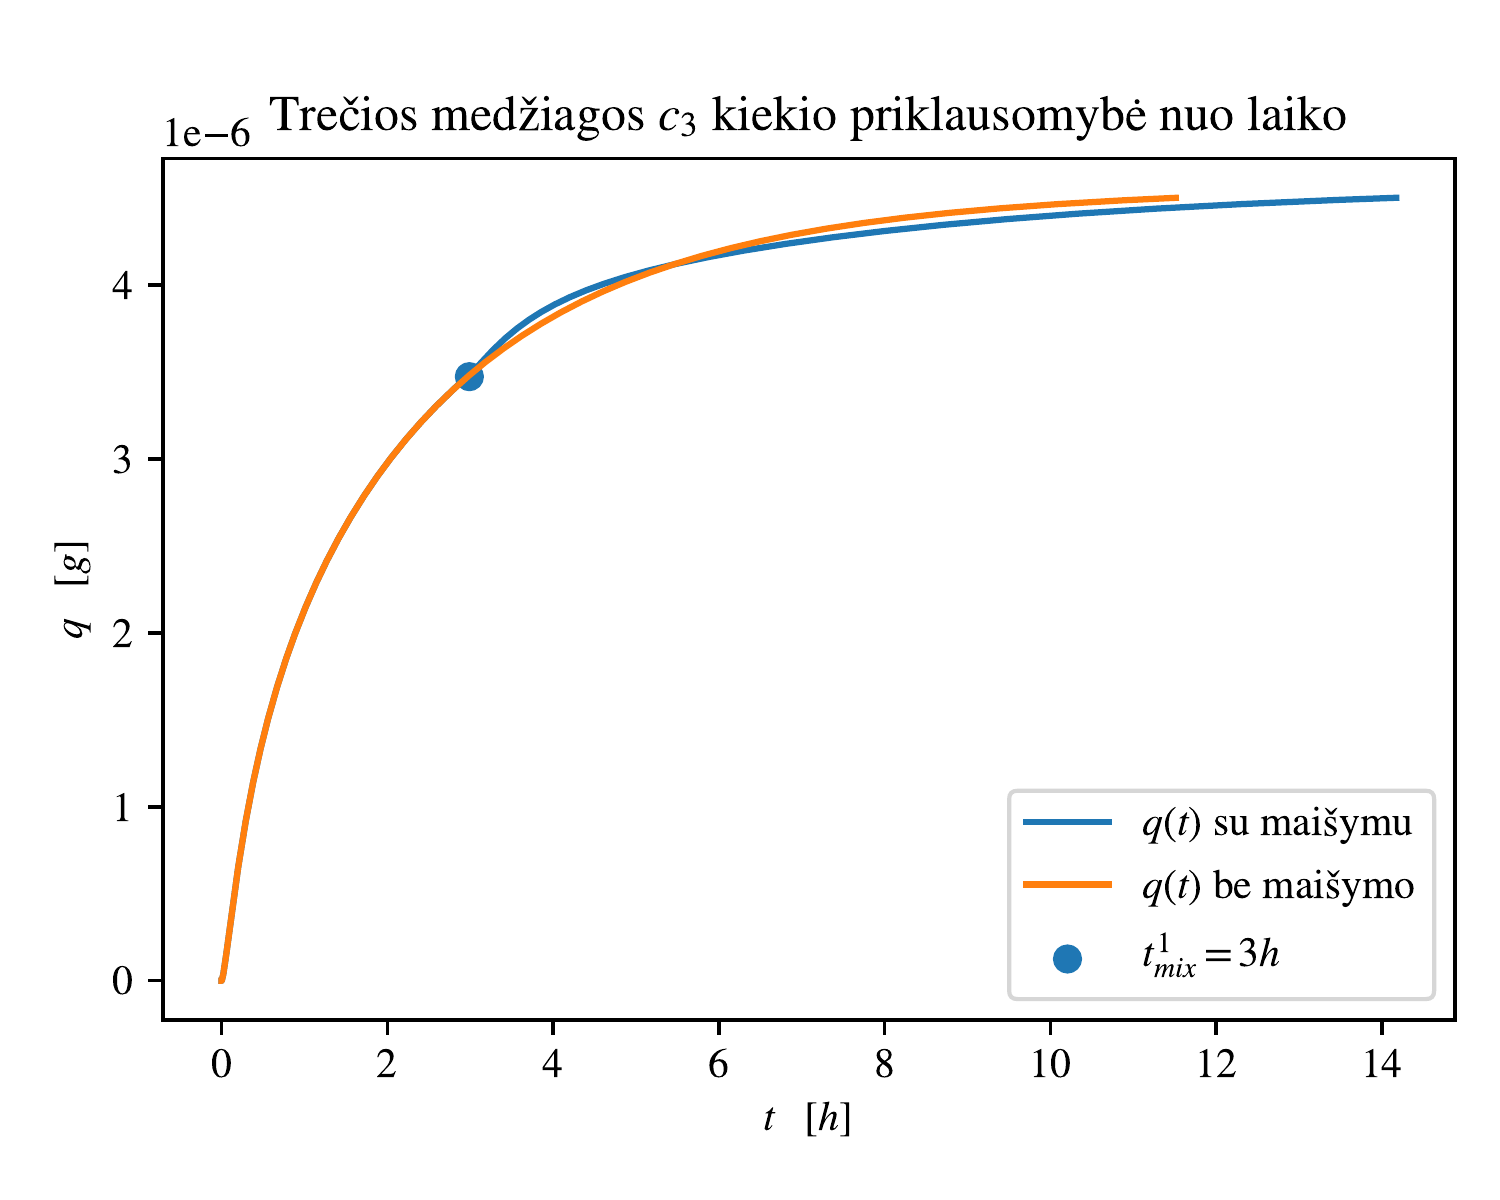
\includegraphics[width=0.5\textwidth]{../paper/assets/bad-mix-qnt-compare-1.png}
    \caption{Kompiuterinio modelio rezultatų palyginimas, kai išmaišymas vyksta ir nevyksta.  }
    \label{bad-mix-qnt-example}
\end{figure}
\ref{bad-mix-qnt-example}-ame pavyzdyje puikiai matosi, kad išmaišymas nepagreitino reakcijos, o ją sulėtino. Reakcijos laikas su išmaišymu yra apytiksliai dvejom su puse valandom ilgesnis. Ši problema atsiranda todėl, kad mes modeliuojame ypač mažą reakcijos erdvės sritį, kurioje susiduria tik 4 mikrodalelės, dėl to nėra daug skirtingų išdėstymų, kada viena sienele galėtų dalintis skirtingų medžiagų dalelės, prie to žinoma prisideda ir faktas, kad šis modelis yra dviejų dimensijų. Eksperimentas parodė, kad nesuveiktų ir statistinis bandymas - vidutinis atsitiktinis išmaišymas taip pat neduoda geresnių rezultatų negu reakcijos modelis be išmaišymų. Dėl šios priežasties apsvarstysime alternatyvų išmaišymo metoda.

\subsection{\enquote{Tobulas} maišymas}

Kad išspręstume atsitiktinio maišymo problemą, modeliuosime \enquote{tobulą} teorinį išmaišymą, kuris turės didžiausią poveikį reakcijos greičiui. Pats maišymo modelis išliks toks pat, tačiau sritis $\Omega_i$ sudėliosime ne atsitiktinai, o sukeisime įstrižai. \enquote{Tobulas} išmaišymas aišku priklauso nuo pradinių sąlygų, o šis galioja tik duotoms pradinėms sąlygoms \eqref{intial-cond}.

\begin{figure}[!h]
\centering
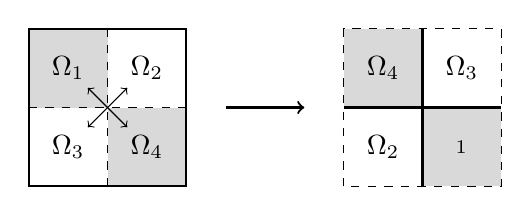
\begin{tikzpicture}
    % Original Grid
    \fill[gray!30] (0,1) rectangle (1, 2);
    \fill[gray!30] (1,0) rectangle (2, 1);
    \draw[<->] (0.75,0.75) -- (1.25,1.25);
    \draw[<->] (1.25,0.75) -- (0.75,1.25);
    \draw[thick] (0,0) rectangle (2,2);
    \draw[dashed] (1,0) -- (1,2);
    \draw[dashed] (0,1) -- (2,1);

    \node at (0.5,1.5) {$\Omega_1$};
    \node at (1.5,1.5) {$\Omega_2$};
    \node at (0.5,0.5) {$\Omega_3$};
    \node at (1.5,0.5) {$\Omega_4$};

    % Arrow
    \draw[->, thick] (2.5,1) -- (3.5,1);

    % Transformed Grid
    \begin{scope}[shift={(4,0)}]
        \fill[gray!30] (0,1) rectangle (1, 2);
        \fill[gray!30] (1,0) rectangle (2, 1);
        
        \draw[dashed] (0,0) rectangle (2,2);
        \draw[thick] (1,0) -- (1,2);
        \draw[thick] (0,1) -- (2,1);

        \node at (0.5,1.5) {$\Omega_4$};
        \node at (1.5,1.5) {$\Omega_3$};
        \node at (0.5,0.5) {$\Omega_2$};
        \node at (1.5,0.5) {$\Oega_1$};
    \end{scope}
\end{tikzpicture}
\caption{\enquote{Tobulo} maišymo transformacija}
\label{perfect-2x2-mix}
\end{figure}
\ref{perfect-2x2-mix}-ame pavyzdyje matoma prieš tai apibūdintą transformacija. Punktyrinės linijos kairėje pusėje žymi sieneles ties kuriomis vyksta reakcija. Šiuo atveju po išmaišymo nėra sričių, kurios turėtų bendrą punktyrinę sienelę, o tai reiškia, kad tokiu būdu sumaišius sritis, visos vidinės sienelės turės didžiausią įmanomą skirtingų medžiagų kontrastą, kuris lems didžiausią įmanomą reakcijos pagreitėjimą.
\newpage
\begin{figure}[h!]
    \centering
    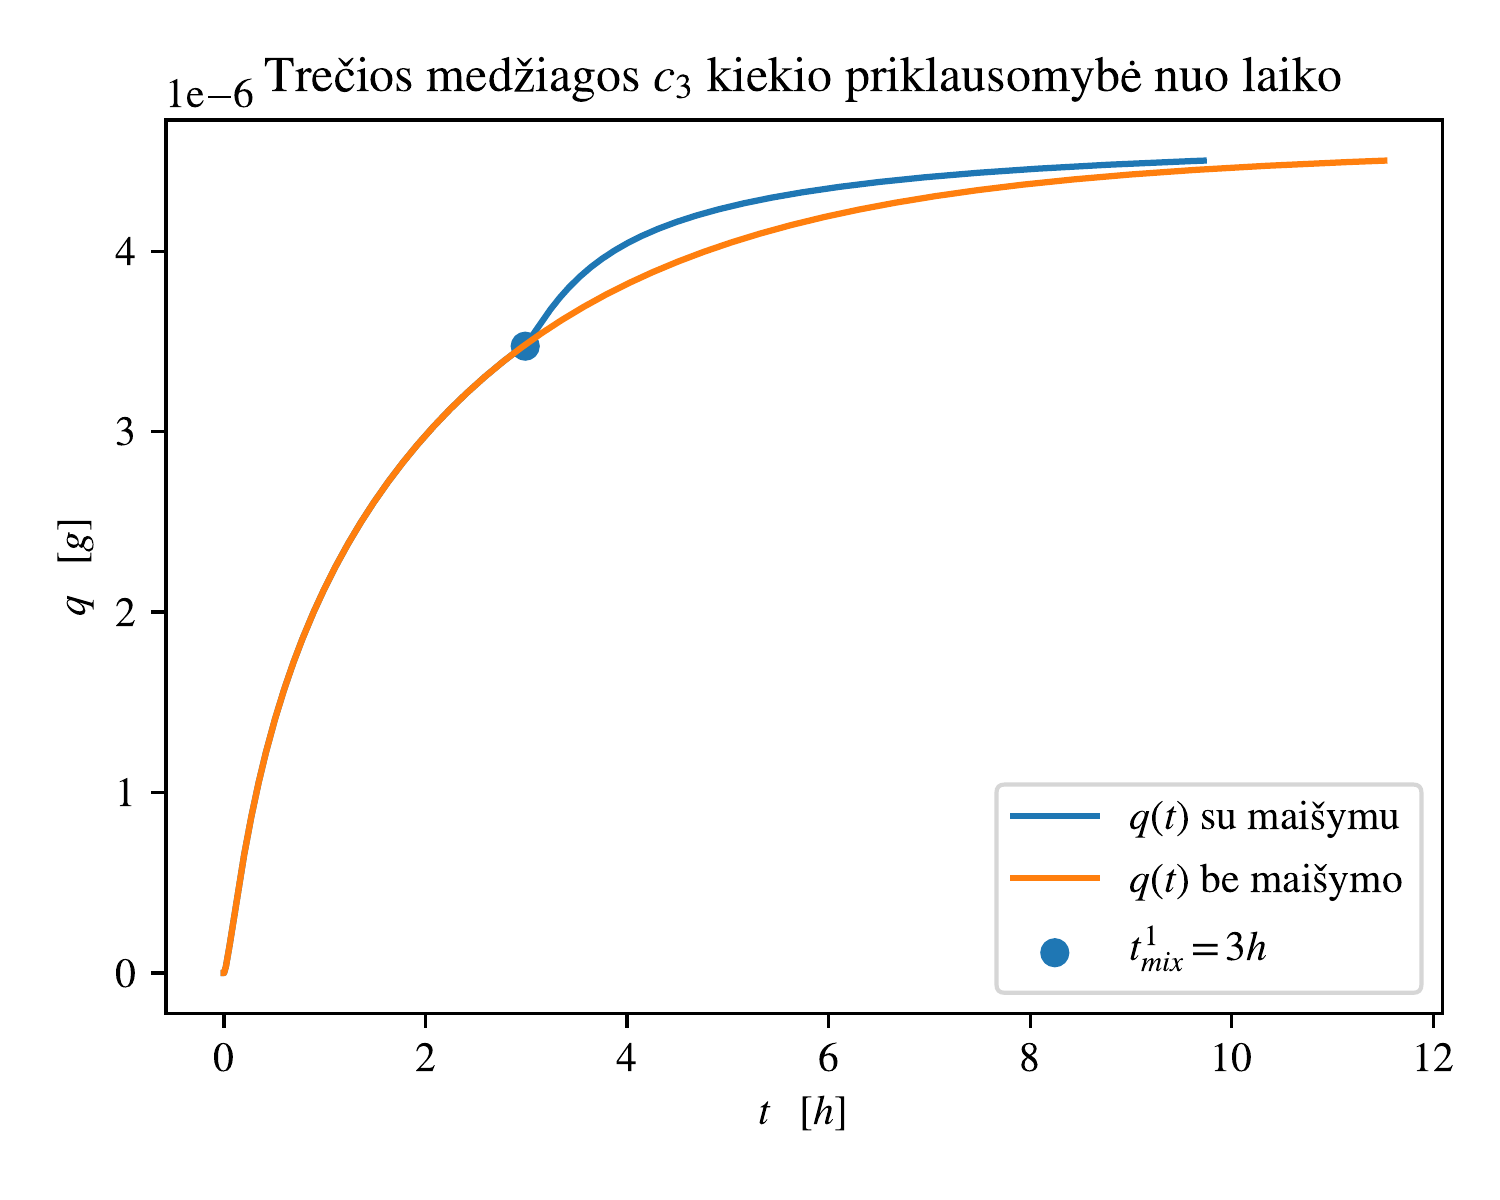
\includegraphics[width=0.5\textwidth]{../paper/assets/optimal-mix-qnt-1.png}

    \caption{Kompiuterinio modelio rezultatų palyginimas tarp reakcijos be išmaišymo ir reakcijos su \enquote{tobulu} išmaišymu.  }

    \label{optimal-mix-qnt}
\end{figure}

Šiuo atveju, \ref{optimal-mix-qnt}-ame pavyzdyje matome, kad dėl \enquote{tobulo} išmaišymo galime matyti šuolį medžiagos kiekyje. Toks maišymas turi teigiamą poveikį reakcijos pabaigos laikui ir labiau atitinka eksperimentinius rezultatus negu atsitiktinis išmaišymas.
Čia galime pasamprotauti, kaip reakcijos pabaigos laikas priklauso nuo išmaišymo laiko - jei išmaišome pradinę konfigūraciją pačioje reakcijos pradžioje, rezultatams tai neturės jokios įtakos ir gausime reakcijos modelį be išmaišymo. Lygiai tas pats nutiktų jei išmaišymas įvyktų ką tik prieš reakcijos pabaigą, tačiau išmaišymas kitais laiko momentais, kaip jau matėme, gali sutrumpinti reakcijos pabaigos laiką. Jei pavaizduotume reakcijos pabaigos laiko priklausomybę nuo išmaišymo laiko, gautume štai tokį grafiką:

\begin{figure}[h!]
    \centering
    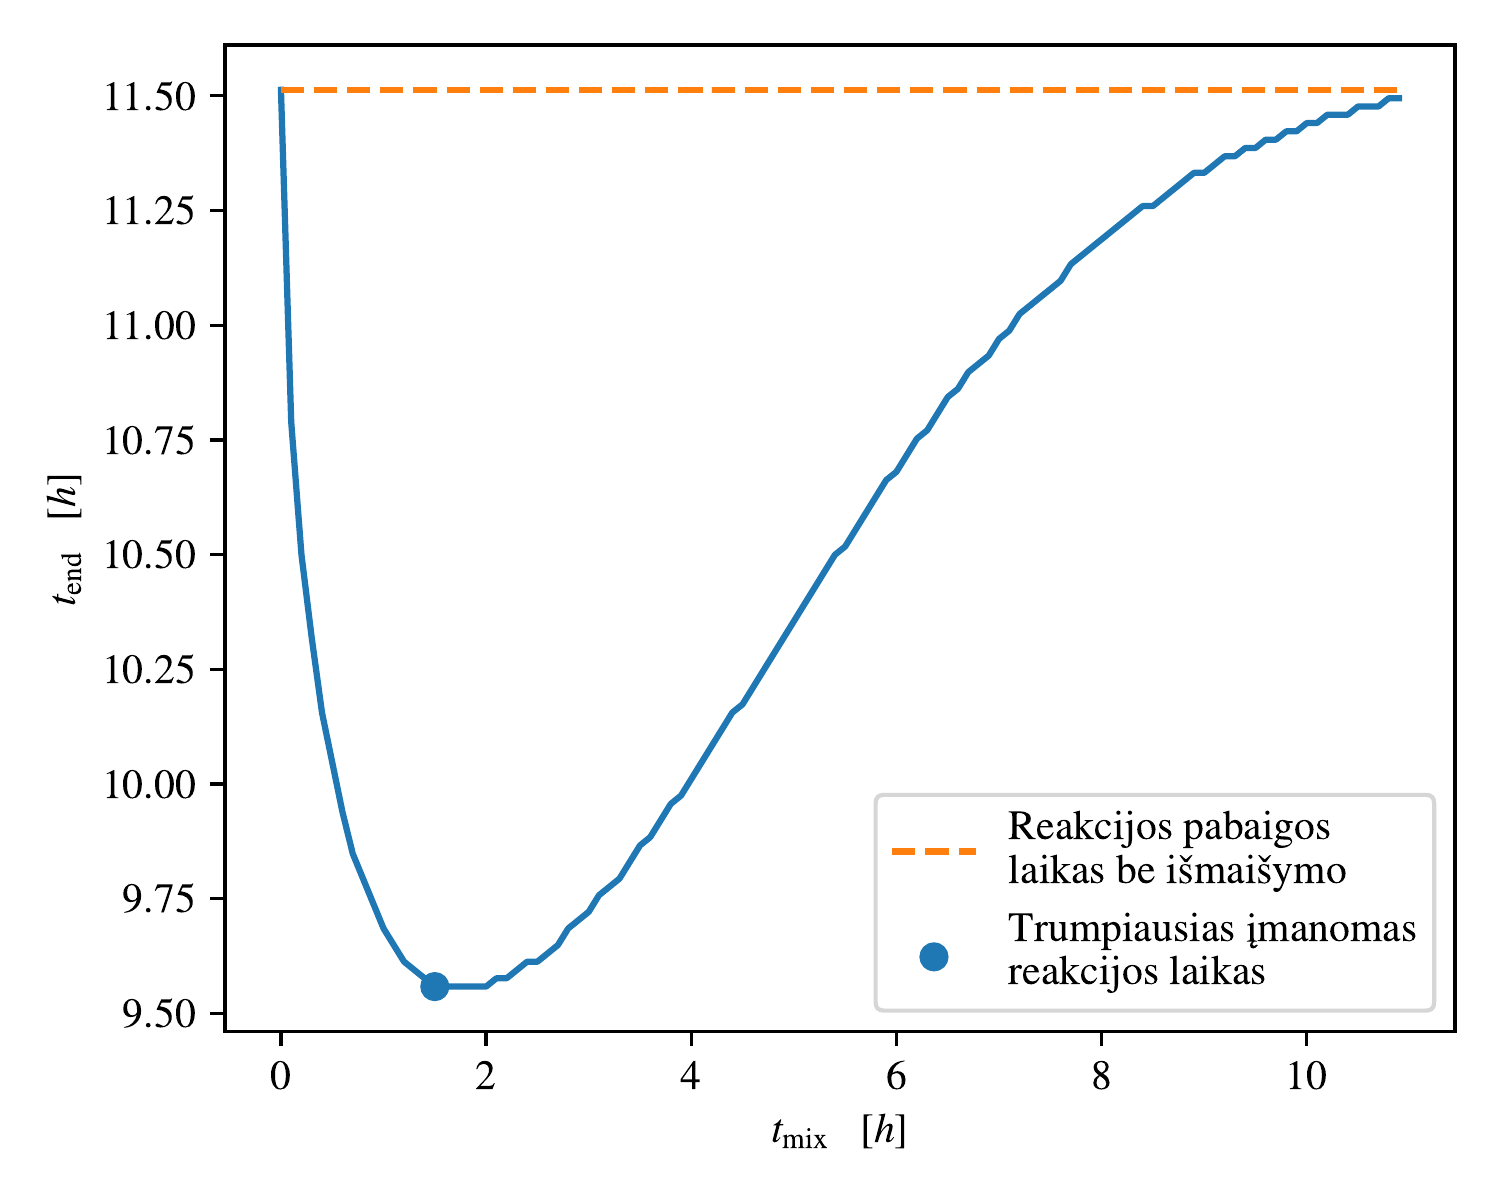
\includegraphics[width=0.5\textwidth]{../paper/assets/mix-end-1.png}

    \caption{Kompiuterinio modelio rezultatai - reakcijos pabaigos laiko priklausomybė nuo išmaišymo laiko. }

    \label{mix-end}
\end{figure}

\ref{mix-end}-ame pavyzdyje matome, kad priklausomybė nėra simetriška, reakcijos pabaigos laikas, kai išmaišymas nevyksta, yra $11h\, 30min$. Optimalus išmaišymo laikas yra $1h\, 30min$ ir tokiu atveju 97\% medžiagų sureaguos per $9h\,33min$.

\subsection{Maišymo modeliavimas didesnėje erdvėje}

Modeliuoti mažą visos reakcijos erdvės sritį užtenka norint gauti tikslias aproksimacijas difuzijos bei reakcijos greičio konstantoms \cite{mackeviciusCloserLookComputer2012}. Tačiau modeliuodami medžiagų išmaišymą neturime priežasties daryti tokios pačios prielaidos. Norint modeliuoti didesnę erdvę, pradines sąlygas reikia atkartoti veidrodiniu principu, tuo galima įsitikinti pažvelgus į \ref{fig:periodic-space}-ą pavyzdį. Modeliuodami didesnę erdvę, ne tik padidės srities plotas, kaip pavaizduota \ref{large-initial-conditions}-ame pavyzdyje, tačiau ir padvigubinsime diskrečių taškų kiekį kiekviena erdvine kryptimi.


\begin{figure}[h!]
\centering
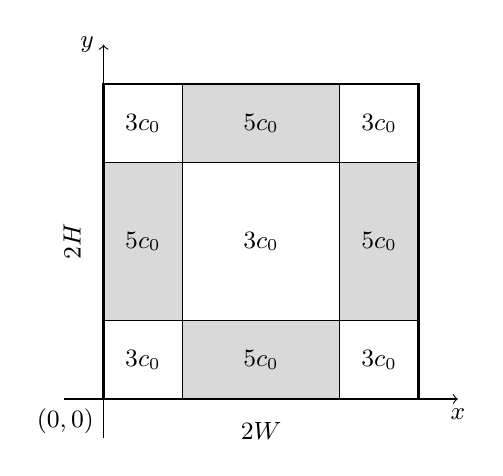
\begin{tikzpicture}
  
    % Fill the boundary cells
    % \fill[gray!30] (0, 3) rectangle (1, 4); % Top-left
    \fill[gray!30] (1, 3) rectangle (3, 4); % Top
    % \fill[gray!30] (3, 3) rectangle (4, 4); % Top-right
    \fill[gray!30] (0, 1) rectangle (1, 3); % Left
    \fill[gray!30] (3, 1) rectangle (4, 3); % Right
    % \fill[gray!30] (0, 0) rectangle (1, 1); % Bottom-left
    \fill[gray!30] (1, 0) rectangle (3, 1); % Bottom
    % \fill[gray!30] (3, 0) rectangle (4, 1); % Bottom-right

    % Draw the outer rectangle
    \draw[thick] (0, 0) rectangle (4, 4);
    \node at (2, -0.4) {\small $2W$};
    \node[rotate=90] at (-0.4, 2) {\small $2H$};

    % Draw the inner rectangle
    \draw[-] (0, 1) -- (4, 1);
    \draw[-] (0, 3) -- (4, 3);
    \draw[-] (1, 0) -- (1, 4);
    \draw[-] (3, 0) -- (3, 4);

    % Labels
    \node at (0.5, 3.5) {\small $3c_0$};
    \node at (2, 3.5) {\small $5c_0$};
    \node at (3.5, 3.5) {\small $3c_0$};

    \node at (0.5, 2) {\small $5c_0$};
    \node at (2, 2) {\small $3c_0$};
    \node at (3.5, 2) {\small $5c_0$};

    \node at (0.5, 0.5) {\small $3c_0$};
    \node at (2, 0.5) {\small $5c_0$};
    \node at (3.5, 0.5) {\small $3c_0$};

    % Coordinate axes
    \draw[->] (-0.5, 0) -- (4.5, 0) node[anchor=north] {\small $x$};
    \draw[->] (0, -0.5) -- (0, 4.5) node[anchor=east] {\small $y$};
    \node[anchor=north east] at (0, 0) {\small $(0,0)$};
\end{tikzpicture}
\caption{ Praplėstos pradinės sąlygos. }

\label{large-initial-conditions}
\end{figure}

Kadangi prieš tai apibrėžtas maišymo modelis yra tinkamas tik įprastoms pradinėms \hbox{sąlygoms \eqref{intial-cond}}, praplėstoms pradinėms sąlygoms reikės atskirai apibrėžti išmaišymą. Eksperimentas parodė, kad net su praplėstomis pradinėmis sąlygomis, atsitiktinio maišymo problema nedingsta - išmaišymas dažniausiai pailgina reakcijos pabaigos laiką. Dėl šios priežasties praplėsime \enquote{tobulo} išmaišymo modelį analogiškai atkartodami jį veidrodžio principu kaip ir pradines sąlygas. 

\begin{figure}[!h]
\centering
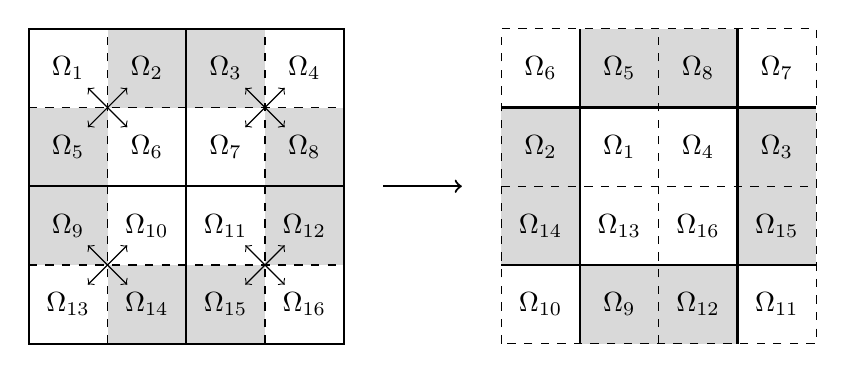
\begin{tikzpicture}
    % Original Grid

    \fill[gray!30] (1, 0) rectangle (3, 1);
    \fill[gray!30] (1, 3) rectangle (3, 4);

    \fill[gray!30] (0, 1) rectangle (1, 3);
    \fill[gray!30] (3, 1) rectangle (4, 3);

    \draw[thick] (0,0) rectangle (2,2);
    \draw[thick] (0,2) rectangle (2,4);
    \draw[thick] (2,0) rectangle (4,2);
    \draw[thick] (2,2) rectangle (4,4);
    \draw[dashed] (1,0) -- (1,4);
    \draw[dashed] (0,1) -- (4,1);
    \draw[dashed] (3,0) -- (3,4);
    \draw[dashed] (0,3) -- (4,3);

    \draw[<->] (0.75,0.75) -- (1.25,1.25);
    \draw[<->] (1.25,0.75) -- (0.75,1.25);

    \draw[<->] (2.75,0.75) -- (3.25,1.25);
    \draw[<->] (3.25,0.75) -- (2.75,1.25);

    \draw[<->] (0.75,2.75) -- (1.25,3.25);
    \draw[<->] (1.25,2.75) -- (0.75,3.25);

    \draw[<->] (2.75,2.75) -- (3.25,3.25);
    \draw[<->] (3.25,2.75) -- (2.75,3.25);

    \node at (0.5,3.5) {$\Omega_1$};
    \node at (1.5,3.5) {$\Omega_2$};
    \node at (0.5,2.5) {$\Omega_5$};
    \node at (1.5,2.5) {$\Omega_6$};

    \node at (2.5,3.5) {$\Omega_3$};
    \node at (3.5,3.5) {$\Omega_4$};
    \node at (2.5,2.5) {$\Omega_7$};
    \node at (3.5,2.5) {$\Omega_8$};

    \node at (0.5,1.5) {$\Omega_9$};
    \node at (1.5,1.5) {$\Omega_{10}$};
    \node at (0.5,0.5) {$\Omega_{13}$};
    \node at (1.5,0.5) {$\Omega_{14}$};

    \node at (2.5,1.5) {$\Omega_{11}$};
    \node at (3.5,1.5) {$\Omega_{12}$};
    \node at (2.5,0.5) {$\Omega_{15}$};
    \node at (3.5,0.5) {$\Omega_{16}$};

    % Arrow
    \draw[->, thick] (4.5,2) -- (5.5,2);

    % Transformed Grid
    \begin{scope}[shift={(6,0)}]
        \fill[gray!30] (1, 0) rectangle (3, 1);
        \fill[gray!30] (1, 3) rectangle (3, 4);

        \fill[gray!30] (0, 1) rectangle (1, 3);
        \fill[gray!30] (3, 1) rectangle (4, 3);

        \draw[dashed] (0,0) rectangle (4,4);

        \draw[dashed] (2,0) -- (2,4);
        \draw[dashed] (0,2) -- (4,2);

        \draw[thick] (1,0) -- (1,4);
        \draw[thick] (0,1) -- (4,1);
        \draw[thick] (3,0) -- (3,4);
        \draw[thick] (0,3) -- (4,3);

        \node at (0.5,3.5) {$\Omega_6$};
        \node at (1.5,3.5) {$\Omega_5$};
        \node at (0.5,2.5) {$\Omega_2$};
        \node at (1.5,2.5) {$\Omega_1$};

        \node at (2.5,3.5) {$\Omega_8$};
        \node at (3.5,3.5) {$\Omega_7$};
        \node at (2.5,2.5) {$\Omega_4$};
        \node at (3.5,2.5) {$\Omega_3$};

        \node at (0.5,1.5) {$\Omega_{14}$};
        \node at (1.5,1.5) {$\Omega_{13}$};
        \node at (0.5,0.5) {$\Omega_{10}$};
        \node at (1.5,0.5) {$\Omega_{9}$};

        \node at (2.5,1.5) {$\Omega_{16}$};
        \node at (3.5,1.5) {$\Omega_{15}$};
        \node at (2.5,0.5) {$\Omega_{12}$};
        \node at (3.5,0.5) {$\Omega_{11}$};
    \end{scope}
\end{tikzpicture}
\caption{\enquote{Tobulo} maišymo transformacija ant praplėstų pradinių sąlygų}
\label{perfect-4x4-mix}
\end{figure}

\ref{perfect-4x4-mix}-ame pavyzdyje matome kaip atrodo \enquote{tobulas} išmaišymas praplėstų pradinių sąlygų atveju. Punktyrinės linijos žymi skirtingų medžiagų bendras sieneles t. y. tas sieneles, ties kuriomis aktyviai vyksta medžiagų reakcija. Paprastos linijos žymi sieneles, ties kuriomis susiduria tos pačios medžiagos sritys arba sieneles, kurios yra nukreiptos į išorę. Toks išmaišymas žymiai padidina reakcijos greitį todėl, kad visos sienelės tarp skirtingų medžiagų yra dar nesureagavusios ir turi dideli koncentracijų kontrastą.

\newpage

\begin{figure}[h!]
    \centering
    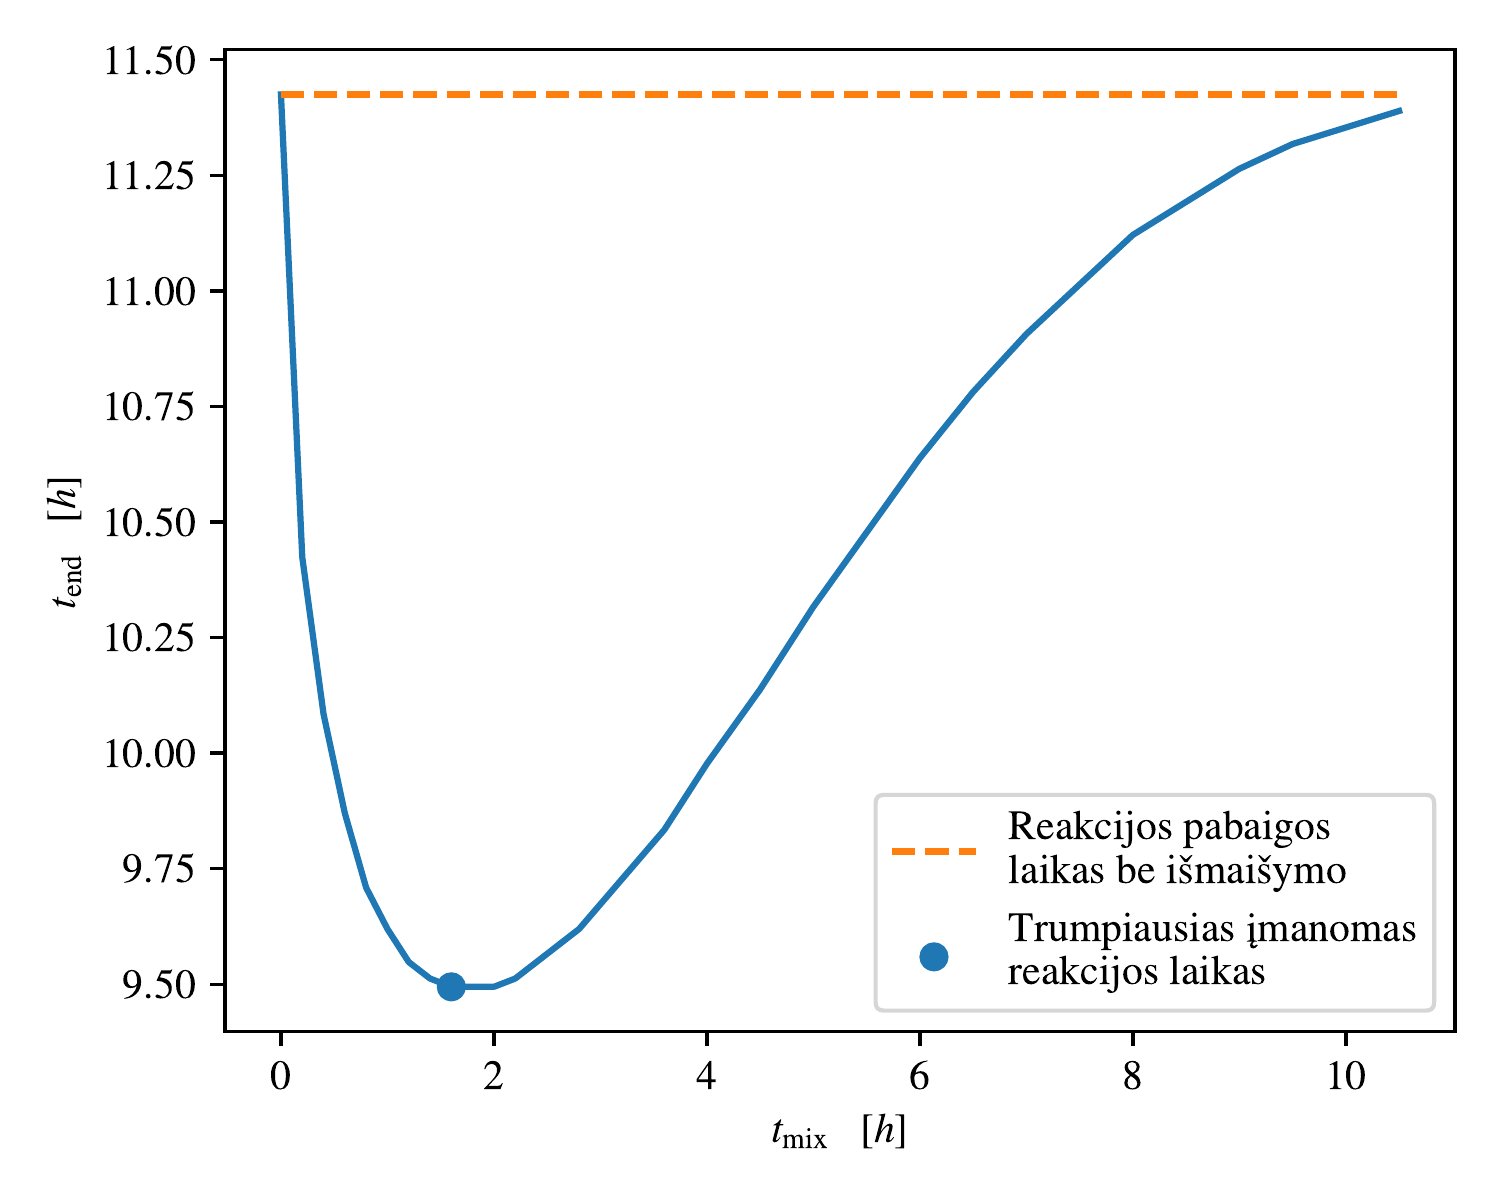
\includegraphics[width=0.5\textwidth]{../paper/assets/mix-end-large-1.png}

    \caption{Reakcijos pabaigos laiko priklausomybė nuo išmaišymo laiko, kai modeliuojamos praplėstos pradinės sąlygos \eqref{large-initial-conditions}. }

    \label{mix-end-large}
\end{figure}

\ref{mix-end-large}-ame matome, kad priklausomybė beveik tokia pati kaip \ref{mix-end}-ame pavyzdyje su nežymiai skirtumais. Kai išmaišymas nevyksta, reakcijos pabaigos laikas yra $11h\,25min$, skirtumas tarp šio ir rezultato su įprastomis pradinėmis sąlygomis yra $5min$. Optimalus išmaišymo laikas šiuo atveju yra $1h\,36min$, skirtumas - $6min$. Reakcijos pabaigos laikas kai medžiagos išmaišomos optimaliu laiku - $9h\,29min$, skirtumas - $4min$.